\documentclass[11pt]{article}

\usepackage[margin=1in]{geometry}
\usepackage{amsmath,amssymb,amsthm}
\usepackage{minted}
\newcommand{\mnt}[1]{{\small\mintinline{java}{#1}}}
\usepackage{tikz}
\usetikzlibrary{arrows}
\usepackage{hyperref}

\theoremstyle{definition}
\newtheorem{thm}{Thm}{}{}
\newtheorem{myDefinition}[thm]{Definition}{\bfseries}{}
\newtheorem{myExample}[thm]{Example}{\bfseries}{}
\newtheorem{myLemma}[thm]{Lemma}{\bfseries}{}
\newtheorem{myTheorem}[thm]{Theorem}{\bfseries}{}

\newcommand{\red}[1]{\textbf{\color{red} #1}}
\newcommand{\N}{\mathbb{N}}
\newcommand{\R}{\mathbb{R}}
\newcommand{\kstar}{^{\textstyle *}}
\newcommand{\sinf}{^\infty}
\newcommand{\serial}{\gg}
\newcommand{\sloop}{\mathsf{loop}}

\newcommand{\sensorId}{\mathit{sensorId}}
\newcommand{\val}{\mathit{val}}
\newcommand{\ts}{\mathit{ts}}
\newcommand{\avg}{\mathit{avg}}
\newcommand{\wndStartTs}{\mathit{wndStartTs}}
\newcommand{\wndEndTs}{\mathit{wndEndTs}}

\begin{document}

\title{COMP 418/518: Homework 4 \\[1ex] \large [Weight of homework: 25\% of the final grade]}
\author{Authors (fill in your names here)}
\date{Due on April 6, 2026 \\ \small (released on March 23, 2026)}

\maketitle

\paragraph{Instructions:}

For this homework, you should work in groups of 3--4 people (i.e., the groups that have been declared and accepted).
%
Only one member of the group should submit on Gradescope.
%
All group members must be included in the submission on the Gradescope system (otherwise no credit will be given).
%
Also specify in your submission file all the members of your group (name and NetID) using the \texttt{\textbackslash authors} macro.
%
The submission must be typed in LaTeX using the provided template.
%
The use of AI systems (including, but not limited to, ChatGPT, Gemini, Copilot, and Claude) is entirely allowed.
%
No discussion or collaboration is allowed outside of the group.
%
Late submissions are not accepted.

\begin{center}
	You should provide \emph{pseudocode} for all the algorithms that you describe.
\end{center}

\paragraph{Grading:}

We will give a 5\% grade bonus to students taking COMP 418. The homework will be graded based on correctness, completeness, and the quality of the provided solutions.

\paragraph{Note:}

Please go over the provided Java source code, because it contains some definitions that are relevant for several questions of the homework. Unless specified otherwise, all the denotations that we consider in the problems are cumulative (i.e., they give the overall output history).

\clearpage % DO NOT REMOVE THIS
\section{The Dataflow Model [110 points]}

We will explore the dataflow model of computation. We consider dataflow graphs where each process (sometimes referred to as node, operator, actor) can be implemented using the following Java interface:
\begin{minted}{java}
public interface Operator<A,B> {
	void start(Sink<B> sink);
	void next(A item, Sink<B> sink);
}

public interface Sink<A> {
	void next(A item);
}
\end{minted}
See the uploaded code for a similar programming model.

We assume that every execution of \mnt{start} and \mnt{next} terminates and thus results in the generation of a \emph{finite} number of output items. Under this assumption, every operator can be described by a \emph{monotone} function $f: A\kstar \to B\kstar$ (cumulative denotation), where $A\kstar$ is the set of all finite words (strings) over $A$. See several lectures that discuss this concept of describing operators (streaming algorithms) using functions.

\subsection{Semantic Characterization of Statelessness [10 points]}

You are asked to give a semantic characterization of the \emph{stateless} operators, that is, those operators that can be implemented without maintaining any state across steps (examples of such operators: \mnt{id}, \mnt{filter}, and \mnt{map}). The operators \mnt{fold} and \mnt{scan}, on the other hand, are stateful. More specifically, you want to characterize the class of (computable) monotone functions $f: A\kstar \to B\kstar$ that admit a stateless implementation. Formulate precisely a property $P(f)$ so that Theorem~\ref{thm:stateless} below holds.

\paragraph{Definition of property $P(f)$:}
%
There exists a function $h: A \to B\kstar$ such that for all $w \in A\kstar$ and all $a \in A$:
\[
	f(w \cdot a) = f(w) \cdot h(a)
\]
In words, the incremental output produced by each new input element $a$ is independent of the prior input history $w$. Equivalently, if we define $\Delta_f(w, a)$ to be the unique string $\delta \in B\kstar$ such that $f(w \cdot a) = f(w) \cdot \delta$ (which exists because $f$ is monotone), then $\Delta_f(u, a) = \Delta_f(v, a)$ for all $u, v \in A\kstar$ and $a \in A$.

\begin{myTheorem}
	\label{thm:stateless}
	Let $f: A\kstar \to B\kstar$ be a computable monotone function. The function $f$ is the cumulative denotation of a stateless operator if and only if $P(f)$.
\end{myTheorem}
\begin{proof}
	$(\Rightarrow)$ Suppose $f$ is the cumulative denotation of a stateless operator. Since the operator is stateless, \mnt{start(sink)} produces a fixed output $s_0 \in B\kstar$ (with no dependence on any mutable state), and for each $a \in A$, \mnt{next(a, sink)} produces output that depends only on $a$, which we denote $h(a) \in B\kstar$. The cumulative denotation satisfies $f(\varepsilon) = s_0$, and for all $w \in A\kstar$ and $a \in A$:
	\[
		f(w \cdot a) = f(w) \cdot h(a).
	\]
	This holds because processing each new element $a$ appends exactly $h(a)$ to the cumulative output, regardless of the prior input history $w$ (since no state is carried across invocations of \mnt{next}). Hence $P(f)$ holds.

	$(\Leftarrow)$ Suppose $P(f)$ holds, i.e., there exists $h: A \to B\kstar$ such that $f(w \cdot a) = f(w) \cdot h(a)$ for all $w \in A\kstar$ and $a \in A$. We construct a stateless operator as follows:
	\begin{itemize}
		\item \mnt{start(sink)}: emit each element of $f(\varepsilon)$ to the sink.
		\item \mnt{next(a, sink)}: emit each element of $h(a)$ to the sink.
	\end{itemize}
	This operator is stateless: neither method accesses or modifies any mutable state that depends on previous inputs. The function $h$ is computable because $h(a) = f(\varepsilon)^{-1} \cdot f(a)$ (removing the prefix $f(\varepsilon)$ from $f(a)$, which is well-defined by monotonicity of $f$).

	Let $f'$ denote the cumulative denotation of this operator. We show $f' = f$ by induction on $|w|$.

	\textbf{Base case:} $f'(\varepsilon) = f(\varepsilon)$ by construction of \mnt{start}.

	\textbf{Inductive step:} Assume $f'(w) = f(w)$ for some $w \in A\kstar$. For any $a \in A$:
	\[
		f'(w \cdot a) = f'(w) \cdot h(a) = f(w) \cdot h(a) = f(w \cdot a),
	\]
	where the first equality follows from the definition of the operator, the second from the inductive hypothesis, and the third from $P(f)$.

	By induction, $f'(w) = f(w)$ for all $w \in A\kstar$. Therefore $f$ is the cumulative denotation of a stateless operator.
\end{proof}

\clearpage % DO NOT REMOVE THIS
\subsection{Translations Between Programming Models [25 points]}

We have used extensively a notation to describe dataflow processes using \mnt{read(channel)} to read from an input channel and \mnt{emit(channel)} to write to an output channel. This programming model was introduced by Kahn in \cite{Kahn1974KPN} and was further elaborated in \cite{KahnMacQ1977}. If you want to learn more about these seminal works you can read the survey \cite{MacQueen2009Kahn} and the notes \cite{Lee2011MoCs} (see reading list on Canvas). Consider the following Kahn process:
\begin{center}
	\begin{tikzpicture}[->, >=to, auto, node distance=1.5cm, semithick, transform shape]
		%
		\footnotesize
		%
		\node (L1) {};
		\node (L2) [below of=L1] {};
		\node (L3) [below of=L2] {};
		\node (M2) [draw, right of=L2, node distance=6cm] {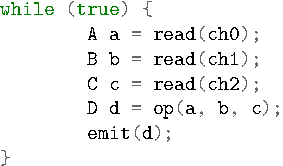
\includegraphics[scale=1.0]{zip3Kahn/zip3Kahn.pdf}};
		\node (R2) [right of=M2, node distance=5cm] {};
		%
		\path (L1) edge[bend left=15] node {\mnt{ch0: A}} (M2);
		\path (L2) edge node {\mnt{ch1: B}} (M2);
		\path (L3) edge[bend right=15] node[swap] {\mnt{ch2: C}} (M2);
		\path (M2) edge node {\mnt{ch: D}} (R2);
		%
	\end{tikzpicture}
\end{center}
Describe the same computation by implementing the \mnt{Zip3} operator of type \mnt{Operator<Or3<A,B,C>,D>}. The three input channels of the Kahn process are encoded using the disjoint union (coproduct) \mnt{Or3<A,B,C>}, which is a straightforward extension of \mnt{Or<A,B>} (see the uploaded code). Fill pseudocode in Figure~\ref{fig:zip3}. You do not have to write actual Java code for this.

\begin{figure}[t!]
	\footnotesize
	\begin{minted}[frame=single]{java}
public class Zip3<A, B, C, D> implements Operator<Or3<A,B,C>, D> {

	private final Func3<A,B,C,D> op;
	private Queue<A> bufA;
	private Queue<B> bufB;
	private Queue<C> bufC;

	public Zip3(Func3<A,B,C,D> op) {
		this.op = op;
		bufA = new LinkedList<>();
		bufB = new LinkedList<>();
		bufC = new LinkedList<>();
	}

	@Override
	public void start(Sink<D> sink) {
		// no output on start
	}

	@Override
	public void next(Or3<A,B,C> item, Sink<D> sink) {
		if (item.isLeft) {
			bufA.add(item.getLeft());
		} else if (item.isMid) {
			bufB.add(item.getMid());
		} else {
			bufC.add(item.getRight());
		}
		while (!bufA.isEmpty() && !bufB.isEmpty()
		       && !bufC.isEmpty()) {
			D d = op.apply(bufA.poll(),
			               bufB.poll(), bufC.poll());
			sink.next(d);
		}
	}
}
\end{minted}
	\caption{The \mnt{Zip3} operator.}
	\label{fig:zip3}
\end{figure}

\begin{figure}[t!]
	\footnotesize
	\begin{minted}[frame=single]{java}
public class Count2 implements Operator<Or<A,A>, Nat> {

	private long count = 0;

	@Override
	public void start(Sink<Nat> sink) { /* do nothing */  }

	@Override
	public void next(Or<A,A> item, Sink<Nat> sink) {
		A a = item.map(x -> x, x -> x);
		count += 1;
		sink.next(count);
	}
}
\end{minted}
	\caption{The \mnt{Count2} operator.}
	\label{fig:count2}
\end{figure}

Consider now the operator \mnt{Count2} of type \mnt{Operator<Or<A,A>,Nat>} that is shown in Figure~\ref{fig:count2}. The input can be thought of as the interleaving of two input channels. Translate \mnt{Count2} into a Kahn process with two input channels (if possible), or prove that it is not possible to do so.

\paragraph{Operator to Kahn process translation:}

\textbf{Claim:} It is \emph{not possible} to translate \mnt{Count2} into a Kahn process with two input channels.

\begin{proof}
	Suppose for contradiction that there exists a Kahn process $P$ with input channels \mnt{ch0: A} and \mnt{ch1: A} and output channel \mnt{ch: Nat} whose cumulative denotation matches that of \mnt{Count2}. That is, the output function satisfies $g(x, y) = 1, 2, \ldots, |x| + |y|$ for all input histories $x$ on \mnt{ch0} and $y$ on \mnt{ch1}.

	A Kahn process is a sequential program whose only input operation is a blocking \mnt{read(ch)} from a specific channel. At the very start of execution (both channels empty), $P$ must attempt to \mnt{read} from either \mnt{ch0} or \mnt{ch1} in order to make progress and eventually produce output.

	\textbf{Case 1:} Suppose $P$ first executes \mnt{read(ch0)}. Consider the input $x = \varepsilon$ (no items on \mnt{ch0}) and $y = b_1$ (one item on \mnt{ch1}). Since $P$ attempts to read from \mnt{ch0} first and \mnt{ch0} is permanently empty, $P$ blocks indefinitely and produces no output. The output of $P$ is $\varepsilon$. However, $g(\varepsilon, b_1) = [1] \neq \varepsilon$, a contradiction.

	\textbf{Case 2:} Suppose $P$ first executes \mnt{read(ch1)}. Then choosing $x = a_1, y = \varepsilon$ yields $g(a_1, \varepsilon) = [1] \neq \varepsilon$, the same contradiction.

	Since these are the only two possible first operations, no Kahn process can compute the function of \mnt{Count2}.

	The fundamental issue is that \mnt{Count2} responds to items arriving on \emph{either} channel, which requires a non-deterministic merge (or \mnt{select}) operation. The Kahn process model only supports deterministic, blocking reads from a single channel, and therefore cannot express this behavior.
\end{proof}

\clearpage % DO NOT REMOVE THIS
\subsection{Denotations [10 points]}

Describe the denotation of \mnt{Zip3} as a function $f: A\kstar \times B\kstar \times C\kstar \to D\kstar$ and the denotation of \mnt{Count2} as a function $g: A\kstar \times A\kstar \to \N\kstar$, where $\N$ is the set of the natural numbers (nonnegative integers).

\paragraph{Solution:}

\textbf{Denotation of Zip3.} The function $f: A\kstar \times B\kstar \times C\kstar \to D\kstar$ is defined by:
\[
	f(a_1 \cdots a_m,\; b_1 \cdots b_n,\; c_1 \cdots c_p) \;=\; d_1 \, d_2 \cdots d_k
\]
where $k = \min(m, n, p)$ and $d_i = \mathit{op}(a_i, b_i, c_i)$ for $i = 1, \ldots, k$. That is, \mnt{Zip3} outputs one element for each complete triple of inputs, processing them in order. If any of the three input channels has fewer items than the others, the excess items on the longer channels are not yet processed (the operator waits for matching items that have not yet arrived).

This function is monotone: if $(x, y, z) \sqsubseteq (x', y', z')$ (componentwise prefix order), then $\min(|x|, |y|, |z|) \leq \min(|x'|, |y'|, |z'|)$ and the corresponding output triples agree on the shared prefix, so $f(x,y,z) \sqsubseteq f(x',y',z')$.

\medskip

\textbf{Denotation of Count2.} The function $g: A\kstar \times A\kstar \to \N\kstar$ is defined by:
\[
	g(a_1 \cdots a_m,\; b_1 \cdots b_n) \;=\; 1,\, 2,\, 3,\, \ldots,\, m + n
\]
That is, the output is the sequence of natural numbers from $1$ to $|x| + |y|$, where $|x| = m$ and $|y| = n$ are the lengths of the two input sequences. \mnt{Count2} ignores the actual values and channel tags of the input items and simply counts the total number of items received.

This function is monotone: if $(x, y) \sqsubseteq (x', y')$, then $|x| + |y| \leq |x'| + |y'|$, so $g(x,y) \sqsubseteq g(x',y')$.

\textbf{Remark:} Although $g$ is a well-defined monotone function, the \emph{timing} of when each count value is emitted depends on the interleaving of the two input channels. This is precisely why \mnt{Count2} cannot be implemented as a Kahn process, as shown in Section~1.2.

\clearpage % DO NOT REMOVE THIS
\subsection{Data Parallelism [25 points]}

In applications that require the processing of massive amounts of data (e.g., data generated by a large number of high-resolution sensors) it is often desirable to exploit \emph{data parallelism}. This is what the distributed data processing systems MapReduce, Spark, Storm and others do. As a simple example of this, consider a pipeline consisting of two \mnt{map} operators:
\begin{center}
	\begin{tikzpicture}[->, >=to, auto, node distance=3cm, semithick, transform shape]
		%
		\footnotesize
		%
		\node (M1) {};
		\node (M2) [draw, right of=M1] {\mnt{map(f)}};
		\node (M3) [draw, right of=M2] {\mnt{map(g)}};
		\node (M4) [right of=M3] {};
		%
		\path (M1) edge node {\mnt{A}} (M2);
		\path (M2) edge node {\mnt{B}} (M3);
		\path (M3) edge node {\mnt{C}} (M4);
	\end{tikzpicture}
\end{center}
We wish to parallelize this pipeline by creating several instances of \mnt{map(f)} and \mnt{map(g)} that compute independently. This is a meaningful transformation when \mnt{f} and \mnt{g} are computationally expensive. This transformation gives rise to dataflow graph of Figure~\ref{fig:data_parallelism}.

\begin{figure}[t]
	\centering
	\begin{tikzpicture}[->, >=to, auto, node distance=1.5cm, semithick, transform shape]
		%
		\footnotesize
		%
		\node (M1) {};
		\node (M2) [draw, right of=M1, node distance=2cm] {\mnt{split}};
		\node (M3) [draw, right of=M2, node distance=3cm] {\mnt{map(f)}};
		\node (M4) [draw, right of=M3, node distance=4cm] {\mnt{map(g)}};
		\node (M5) [draw, right of=M4, node distance=3cm] {\mnt{merge}};
		\node (M6) [right of=M5, node distance=2cm] {};
		%
		\node (T3) [draw, above of=M3] {\mnt{map(f)}};
		\node (T4) [draw, above of=M4] {\mnt{map(g)}};
		%
		\node (B3) [draw, below of=M3] {\mnt{map(f)}};
		\node (B4) [draw, below of=M4] {\mnt{map(g)}};
		%
		\path (M1) edge node {\mnt{A}} (M2);
		\path (M2) edge[bend left] node {\mnt{A}} (T3);
		\path (M2) edge node {\mnt{A}} (M3);
		\path (M2) edge[bend right] node[swap] {\mnt{A}} (B3);
		\path (T3) edge node {\mnt{B}} (T4);
		\path (T3) edge (M4);
		\path (T3) edge (B4);
		\path (M3) edge (T4);
		\path (M3) edge (M4);
		\path (M3) edge (B4);
		\path (B3) edge (T4);
		\path (B3) edge (M4);
		\path (B3) edge node[swap] {\mnt{B}} (B4);
		\path (T4) edge[bend left] node {\mnt{C}} (M5);
		\path (M4) edge node {\mnt{C}} (M5);
		\path (B4) edge[bend right] node[swap] {\mnt{C}} (M5);
		\path (M5) edge node {\mnt{C}} (M6);
	\end{tikzpicture}
	\caption{Extracting data parallelism from a simple pipeline of stateless operators.}
	\label{fig:data_parallelism}
\end{figure}

Describe each of the nodes (processes) of the dataflow graph of Figure~\ref{fig:data_parallelism}. You can assume that every communication channel is reliable (no messages are lost) and behaves like a FIFO buffer. Make sure that the behavior of the graph of Figure~\ref{fig:data_parallelism} (in terms of the input/output function) is exactly the same as the behavior of the original pipeline. Does this require making any noteworthy changes to the graph? You may have to introduce new notation for writing pseudocode that describes the nodes. Try to make your notation intuitive and explain the aspects that are not obvious. You do not have to restrict yourself to Kahn processes for the code that runs on each node.

\paragraph{Solution:}

We describe each node of the dataflow graph in Figure~\ref{fig:data_parallelism}. Let $N = 3$ denote the degree of parallelism. To ensure that the parallel graph has the same input/output behavior as the original pipeline \mnt{map(f) >> map(g)}, we use round-robin distribution and collection, which implicitly preserves the ordering of items without requiring explicit sequence numbers.

We use the following notation: \mnt{read(ch)} blocks until an item is available on channel \mnt{ch} and returns it; \mnt{emit(item, ch)} sends an item on channel \mnt{ch}. All channels are FIFO.

\paragraph{split node.} The \mnt{split} node distributes input items to the three \mnt{map(f)} instances in round-robin fashion. Let $\mathit{out}[0]$, $\mathit{out}[1]$, $\mathit{out}[2]$ be the three output channels.

\begin{minted}{java}
// split: 1 input channel (in), 3 output channels (out[0..2])
lane = 0;
while (true) {
    A a = read(in);
    emit(a, out[lane]);
    lane = (lane + 1) % 3;
}
\end{minted}

Item $i$ (0-indexed) is sent to lane $i \bmod 3$. Thus lane 0 receives items $0, 3, 6, \ldots$; lane 1 receives items $1, 4, 7, \ldots$; and lane 2 receives items $2, 5, 8, \ldots$

\paragraph{map(f) instance $i$ ($i \in \{0, 1, 2\}$).} Each \mnt{map(f)} instance reads items from its input channel (from \mnt{split}), applies $f$, and sends the result to \mnt{map(g)}$_i$ on the lane-local output channel.

\begin{minted}{java}
// map(f) instance i: input from split, output to map(g)[i]
while (true) {
    A a = read(in);
    B b = f(a);
    emit(b, out);
}
\end{minted}

\paragraph{map(g) instance $i$ ($i \in \{0, 1, 2\}$).} Each \mnt{map(g)} instance reads intermediate results from \mnt{map(f)}$_i$, applies $g$, and sends the result to the \mnt{merge} node.

\begin{minted}{java}
// map(g) instance i: input from map(f)[i], output to merge
while (true) {
    B b = read(in);
    C c = g(b);
    emit(c, out);
}
\end{minted}

\paragraph{merge node.} The \mnt{merge} node collects outputs from the three \mnt{map(g)} instances and emits them in the original input order. Since \mnt{split} distributes items round-robin, the order can be reconstructed by reading from the three input channels in the same round-robin fashion.

\begin{minted}{java}
// merge: 3 input channels (in[0..2]), 1 output channel (out)
lane = 0;
while (true) {
    C c = read(in[lane]);
    emit(c, out);
    lane = (lane + 1) % 3;
}
\end{minted}

\paragraph{Correctness.} The input sequence $a_0, a_1, a_2, a_3, a_4, a_5, \ldots$ is distributed by \mnt{split} so that lane $i$ receives items $a_i, a_{i+3}, a_{i+6}, \ldots$ Each \mnt{map(f)} and \mnt{map(g)} instance preserves the FIFO order. After applying $f$ and $g$ on each lane, lane $i$ outputs $g(f(a_i)), g(f(a_{i+3})), g(f(a_{i+6})), \ldots$ The \mnt{merge} reads round-robin (lane 0, 1, 2, 0, 1, 2, \ldots), producing:
\[
	g(f(a_0)),\; g(f(a_1)),\; g(f(a_2)),\; g(f(a_3)),\; g(f(a_4)),\; g(f(a_5)),\; \ldots
\]
This is exactly the output of the original pipeline \mnt{map(f) >> map(g)}.

\paragraph{Noteworthy changes to the graph.}

\begin{enumerate}
	\item \textbf{Simplification of cross-connections.} The graph in Figure~\ref{fig:data_parallelism} shows all nine connections between the \mnt{map(f)} and \mnt{map(g)} layers (every \mnt{map(f)} instance is connected to every \mnt{map(g)} instance). However, with round-robin distribution, each \mnt{map(f)}$_i$ only needs to communicate with \mnt{map(g)}$_i$ (lane-local routing). The six cross-lane connections are unnecessary and should be removed. If they were used and each \mnt{map(f)} instance broadcast its output to all three \mnt{map(g)} instances, items would be processed multiple times by different \mnt{map(g)} instances, producing incorrect (duplicated) output. Alternatively, if the cross-connections are retained, a routing mechanism must ensure each item reaches exactly one \mnt{map(g)} instance.

	\item \textbf{All nodes are deterministic Kahn processes.} A notable advantage of the round-robin split/merge approach is that all nodes (including \mnt{merge}) are deterministic Kahn processes. The \mnt{merge} does not require a non-deterministic \mnt{select} operation---it simply reads from channels in a fixed round-robin order. This would not be possible if the cross-connections were used with arbitrary routing, since \mnt{map(g)} instances would then need to read from multiple input channels non-deterministically.

	\item \textbf{Finite stream handling.} If the input stream has $n$ items where $n$ is not a multiple of 3, the lanes will have unequal numbers of items ($\lceil n/3 \rceil$ vs.\ $\lfloor n/3 \rfloor$). The round-robin merge will correctly output all $n$ items before blocking on the next read from a shorter lane. This blocking is the standard Kahn-model behavior for the end of a finite stream and does not affect correctness.
\end{enumerate}

\clearpage % DO NOT REMOVE THIS
\subsection{Disorder and Watermarks [40 points]}

Consider an IoT application that requires collecting data from a large and physically distributed collection of smart sensors. All sensor streams are sent to a centralized location (``server'') for processing. Because of the physical distribution, the data can arrive disordered. The server sees a single input stream of data items of the form $(\sensorId, \val, \ts): \N \times \R \times \N$, where $\sensorId: \N$ is a unique identifier for a sensor, $\val: \R$ is the sensor measurement, and $\ts: \N$ is a timestamp that measures time in msec (milliseconds). The data items in the input stream may be \emph{disordered} with respect to the timestamp. So, we \emph{cannot} expect in general that the data will appear in non-decreasing timestamp order.

We define the \emph{watermark} of the input stream to be the maximum timestamp seen so far\footnote{Similar notions of watermarks are considered in many data stream processing systems. For example, see \url{https://learn.microsoft.com/en-us/azure/stream-analytics/stream-analytics-time-handling} and \url{https://www.databricks.com/blog/feature-deep-dive-watermarking-apache-spark-structured-streaming}.}. We make a \emph{bounded lateness} assumption, namely that each data item should be at most $T \geq 0$ time units behind the watermark. That is, if $(\sensorId, \val, \ts)$ is the current data item and $t$ is the current watermark, then it should hold that $t - \ts \leq T$.

We want to compute the \emph{tumbling window average} of the measurement values. Suppose that $W > 0$ is the length of the window. For each time interval $[0, W), [W, 2W), [2W, 3W), \ldots$ we want to output the average value of all measurements that belong to the interval according to their timestamp. The output should be of the form $(\avg, \wndStartTs, \wndEndTs): \R \times \N \times \N$, where $\avg: \R$ is the average measurement of the window, $\N$ is the start time of the window, and $\N$ is the end time of the window. E.g., if $y_0$ is the average of the window $[0, W)$, then the output should be $(y_0, 0, W - 1)$.
\begin{center}
	\begin{tikzpicture}[->, >=to, auto, node distance=6cm, semithick, transform shape]
		%
		\footnotesize
		%
		\node (M1) {};
		\node (M2) [draw, right of=M1] {\mnt{tumbling-window(W, val, average)}};
		\node (M3) [right of=M2] {};
		%
		\path (M1) edge node {$\N \times \R \times \N$} (M2);
		\path (M2) edge node {$\R \times \N \times \N$} (M3);
	\end{tikzpicture}
\end{center}
You should emit the output for a window as early as possible, i.e., as soon as it becomes apparent that no other measurement of the window will be seen in the future (recall the bounded lateness assumption).

Provide detailed streaming pseudocode for the most efficient implementation of this tumbling window operator that you can think of. Discuss the memory and time-per-item complexity of your implementation.

\paragraph{Solution:}

\subparagraph{Approach.} We maintain a watermark (maximum timestamp seen so far) and accumulate per-window statistics (sum and count of measurement values). When the watermark advances far enough that no more items can arrive for a given window (under the bounded lateness assumption), we close that window and emit its average.

\subparagraph{Window assignment.} An item with timestamp $\ts$ belongs to window $k = \lfloor \ts / W \rfloor$, which covers the time interval $[kW, (k+1)W)$.

\subparagraph{Closing condition.} Under the bounded lateness assumption, any future item has timestamp $\ts \geq \text{watermark} - T$. This follows because the watermark is non-decreasing: after the current watermark reaches $w$, any subsequently arriving item with timestamp $\ts'$ satisfies $w' - \ts' \leq T$ where $w' \geq w$ is the watermark at the time of that item's arrival. If $\ts' \geq w'$, then $\ts' \geq w' \geq w \geq w - T$. If $\ts' < w'$, then $\ts' \geq w' - T \geq w - T$. In both cases, $\ts' \geq w - T$.

Window $k$ covers timestamps up to $(k+1)W - 1$. Therefore, window $k$ can be safely closed when no future item can have a timestamp in $[kW, (k+1)W)$, which occurs when:
\[
	\text{watermark} - T \geq (k+1)W \quad \Longleftrightarrow \quad \text{watermark} \geq (k+1)W + T
\]
At this point, all future items will have timestamps $\geq (k+1)W$, placing them in window $k+1$ or later.

\subparagraph{Pseudocode.}

\begin{minted}[frame=single]{java}
class TumblingWindowAvg
    implements Operator<(Nat, Real, Nat), (Real, Nat, Nat)> {

  final int W; // window size (msec)
  final int T; // max lateness (msec)

  // State
  int watermark = -1;
  int nextToClose = 0; // smallest window id not yet closed
  HashMap<Integer, Double>  sumMap   = new HashMap<>();
  HashMap<Integer, Integer> countMap = new HashMap<>();

  void start(Sink sink) { /* no output on start */ }

  void next((int sensorId, double val, int ts), Sink sink) {
    // 1. Update watermark
    watermark = max(watermark, ts);

    // 2. Assign item to its tumbling window
    int wid = ts / W; // floor division = window id

    // 3. Update the window's running sum and count
    if (!sumMap.containsKey(wid)) {
      sumMap.put(wid, 0.0);
      countMap.put(wid, 0);
    }
    sumMap.put(wid, sumMap.get(wid) + val);
    countMap.put(wid, countMap.get(wid) + 1);

    // 4. Emit all closeable windows in chronological order
    while ((nextToClose + 1) * W + T <= watermark) {
      if (sumMap.containsKey(nextToClose)) {
        double avg   = sumMap.get(nextToClose)
                     / countMap.get(nextToClose);
        int wndStart = nextToClose * W;
        int wndEnd   = (nextToClose + 1) * W - 1;
        sink.next((avg, wndStart, wndEnd));
        sumMap.remove(nextToClose);
        countMap.remove(nextToClose);
      }
      // Skip empty windows (no items fell in this interval)
      nextToClose++;
    }
  }
}
\end{minted}

\subparagraph{Detailed explanation.}

\begin{enumerate}
	\item \textbf{Watermark update (line 18):} On each incoming item, we update the watermark to be the maximum of the current watermark and the item's timestamp. The watermark is monotonically non-decreasing.

	\item \textbf{Window assignment (line 21):} The window ID is computed as $\lfloor \ts / W \rfloor$, placing the item in the tumbling window $[kW, (k+1)W)$ where $k = \lfloor \ts / W \rfloor$.

	\item \textbf{Accumulator update (lines 23--28):} We maintain a running sum and count for each active window. This allows computing the average when the window closes, \emph{without storing individual data items}. Only two numbers per window are needed.

	\item \textbf{Window closing (lines 31--40):} We maintain a variable \mnt{nextToClose} that tracks the smallest window ID that has not yet been closed. After each watermark update, we check in a while loop whether pending windows can be closed. A window with ID $k$ is closeable when $(k + 1) \cdot W + T \leq \text{watermark}$.

	      If the window accumulated items, we compute and emit the average. Windows with no items are silently skipped (no average to emit). The \mnt{nextToClose} pointer advances monotonically, ensuring windows are emitted in chronological order and each window is processed at most once.

	\item \textbf{Earliest possible emission:} The output for each window is emitted immediately when the closing condition is first satisfied by a watermark advance. This is the earliest possible moment: before this point, the bounded lateness assumption still allows items to arrive for the window, so we cannot emit sooner without risking an incorrect average.

	\item \textbf{No late items reach closed windows:} Under the bounded lateness assumption, once we close window $k$ (when $\text{watermark} \geq (k+1)W + T$), any future item satisfies $\ts \geq \text{watermark} - T \geq (k+1)W$. Such items belong to window $k+1$ or later, so they never need to update a closed window. The invariant $\textit{wid} \geq \textit{nextToClose}$ always holds.
\end{enumerate}

\subparagraph{Complexity analysis.}

\begin{itemize}
	\item \textbf{Time per item: $O(1)$ amortized.} The watermark update, window assignment, and accumulator update are each $O(1)$ (hash map operations with expected constant-time lookup). The while loop for closing windows runs at most once per window over the entire execution of the stream. Since each window is closed exactly once, the total closing work across all $n$ items is bounded by the total number of windows (at most $n$ windows, but typically far fewer). By an amortized argument, the cost is $O(1)$ per item.

	\item \textbf{Memory: $O(T/W + 1)$.} At any point, the active (not yet closed) windows are those covering timestamps in the range $[\text{watermark} - T,\; \text{watermark}]$. The number of distinct tumbling windows that intersect this range is at most:
	      \[
		      \left\lfloor \frac{T}{W} \right\rfloor + 2 \;=\; O\!\left(\frac{T}{W} + 1\right)
	      \]
	      Each window stores only a sum and a count ($O(1)$ space per window), so the total memory for window accumulators is $O(T/W + 1)$. Importantly, we do \emph{not} store individual data items---only aggregate statistics. The \mnt{sensorId} field is not used for the global average computation.

	      When $T < W$ (lateness is less than one window), at most 2 windows are active at any time, giving $O(1)$ memory. When $T \gg W$ (high lateness relative to window size), many windows may be simultaneously active, reflecting the inherent cost of handling disorder.
\end{itemize}

\clearpage % DO NOT REMOVE THIS
\section{Denotational Semantics of Kahn Process Networks [40 points]}

\begin{myLemma}
	Let $A$ and $B$ be $\omega$-CPOs. Then, $A \times B$ is an $\omega$-CPO.
\end{myLemma}
\begin{proof}
	We equip $A \times B$ with the componentwise partial order: $(a_1, b_1) \sqsubseteq (a_2, b_2)$ iff $a_1 \sqsubseteq_A a_2$ and $b_1 \sqsubseteq_B b_2$. We verify the two requirements of an $\omega$-CPO.

	\textbf{Least element.} Since $A$ and $B$ are $\omega$-CPOs, they have least elements $\bot_A$ and $\bot_B$ respectively. We claim $(\bot_A, \bot_B)$ is the least element of $A \times B$. For any $(a, b) \in A \times B$, we have $\bot_A \sqsubseteq_A a$ and $\bot_B \sqsubseteq_B b$, so $(\bot_A, \bot_B) \sqsubseteq (a, b)$.

	\textbf{Least upper bounds of $\omega$-chains.} Let $(a_0, b_0) \sqsubseteq (a_1, b_1) \sqsubseteq (a_2, b_2) \sqsubseteq \cdots$ be an $\omega$-chain in $A \times B$. By the definition of the componentwise order, this gives rise to two $\omega$-chains:
	\[
		a_0 \sqsubseteq_A a_1 \sqsubseteq_A a_2 \sqsubseteq_A \cdots \quad \text{in } A, \qquad b_0 \sqsubseteq_B b_1 \sqsubseteq_B b_2 \sqsubseteq_B \cdots \quad \text{in } B.
	\]
	Since $A$ is an $\omega$-CPO, the chain $(a_n)_{n \geq 0}$ has a least upper bound $a = \bigsqcup_n a_n$ in $A$. Since $B$ is an $\omega$-CPO, the chain $(b_n)_{n \geq 0}$ has a least upper bound $b = \bigsqcup_n b_n$ in $B$.

	We claim that $(a, b) = \bigsqcup_n (a_n, b_n)$ in $A \times B$.

	\emph{Upper bound:} For all $n \geq 0$, we have $a_n \sqsubseteq_A a$ and $b_n \sqsubseteq_B b$, so $(a_n, b_n) \sqsubseteq (a, b)$.

	\emph{Least upper bound:} Let $(a', b')$ be any upper bound of the chain, i.e., $(a_n, b_n) \sqsubseteq (a', b')$ for all $n$. Then $a_n \sqsubseteq_A a'$ for all $n$, so $a'$ is an upper bound of the chain $(a_n)_{n \geq 0}$ in $A$. Since $a = \bigsqcup_n a_n$ is the \emph{least} upper bound, we have $a \sqsubseteq_A a'$. By the same argument, $b \sqsubseteq_B b'$. Therefore $(a, b) \sqsubseteq (a', b')$.

	This shows that every $\omega$-chain in $A \times B$ has a least upper bound. Hence $A \times B$ is an $\omega$-CPO.
\end{proof}

\begin{myLemma}
	Let $A$, $B$ and $C$ be $\omega$-CPOs. Suppose that $f: A \to B$ and $g: B \to C$ are $\omega$-continuous. Then, the serial composition $f \serial g: A \to C$ is $\omega$-continuous. Recall from the lectures that $(f \serial g)(a) = g(f(a))$ for every $a \in A$.
\end{myLemma}
\begin{proof}
	We need to show that $f \serial g$ is $\omega$-continuous, i.e., (1) monotone and (2) preserving least upper bounds of $\omega$-chains.

	\textbf{Monotonicity.} Let $a_1 \sqsubseteq_A a_2$. Since $f$ is $\omega$-continuous, it is monotone, so $f(a_1) \sqsubseteq_B f(a_2)$. Since $g$ is $\omega$-continuous, it is monotone, so $g(f(a_1)) \sqsubseteq_C g(f(a_2))$. Therefore $(f \serial g)(a_1) \sqsubseteq_C (f \serial g)(a_2)$.

	\textbf{Preservation of $\omega$-chain suprema.} Let $a_0 \sqsubseteq a_1 \sqsubseteq a_2 \sqsubseteq \cdots$ be an $\omega$-chain in $A$. We compute:
	\begin{align*}
		(f \serial g)\!\left(\bigsqcup_n a_n\right)
		 & = g\!\left(f\!\left(\bigsqcup_n a_n\right)\right)                                                  \\
		 & = g\!\left(\bigsqcup_n f(a_n)\right)              & \text{($f$ is $\omega$-continuous)}            \\
		 & = \bigsqcup_n g(f(a_n))                           & \text{($g$ is $\omega$-continuous; see below)} \\
		 & = \bigsqcup_n (f \serial g)(a_n)
	\end{align*}

	In the third step, we applied the $\omega$-continuity of $g$ to the sequence $f(a_0), f(a_1), f(a_2), \ldots$ in $B$. This is indeed an $\omega$-chain because $f$ is monotone: $a_i \sqsubseteq_A a_{i+1}$ implies $f(a_i) \sqsubseteq_B f(a_{i+1})$ for all $i \geq 0$. Therefore the $\omega$-continuity of $g$ applies, yielding $g\!\left(\bigsqcup_n f(a_n)\right) = \bigsqcup_n g(f(a_n))$.

	Hence $f \serial g$ is $\omega$-continuous.
\end{proof}

We will consider now the \textbf{\em semantics of feedback} using an interesting example. Consider the Kahn process shown below:
\begin{center}
	\begin{tikzpicture}[->, >=to, auto, node distance=1.5cm, semithick, transform shape]
		%
		\footnotesize
		%
		\node (L1) {};
		\node (L2) [below of=L1] {};
		\node (L3) [below of=L2] {};
		\node (M2) [draw, right of=L2, node distance=6cm] {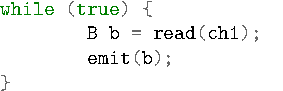
\includegraphics[scale=1.0]{projKahn/projKahn.pdf}};
		\node (R2) [right of=M2, node distance=5cm] {};
		%
		\path (L1) edge[bend left=10] node {\mnt{ch0: A}} (M2);
		\path (L3) edge[bend right=10] node[swap] {\mnt{ch1: B}} (M2);
		\path (M2) edge node {\mnt{ch: B}} (R2);
		%
	\end{tikzpicture}
\end{center}
The (cumulative) input/output behavior of this process can be described by an $\omega$-continuous function $f: A\sinf \times B\sinf \to B\sinf$. Describe the function $f$ and the function $\sloop(f): A\sinf \to B\sinf$ ($\sloop$ is feedback composition, as defined in the lectures).

\paragraph{Solution:}

\red{Fill me in.}

\clearpage % DO NOT REMOVE THIS
\section{ToyDSL [100 points]}

Download the Java project form Canvas. Carefully read all the provided code in order to understand the programming model that we consider. Implement the ToyDSL domain-specific language using the included instructions. Your implementation should pass all included unit tests. If there is anything that you would like to clarify, please do so below.

\subsection*{Solution}

\red{Fill me in.}


\bibliographystyle{plain}
\bibliography{refs}

\end{document}